%% Beamer-ported version of mru.tex ==
%% 
%% Original created 05-10-2008; ported to Beamer July 2025
\documentclass{beamer}

\usepackage{xcolor}
\usetheme{Copenhagen}  % Change to Madrid, Copenhagen, etc., for fancier look
% Define custom colors
\definecolor{electricblue}{RGB}{0,191,255} % Electric blue
\definecolor{creamyblue}{RGB}{173,216,230} % Creamy blue
\newcommand{\red}[1]{\textcolor{red}{#1}}
%\setbeamercolor{structure}{fg=electricblue} % Apply electric blue
\setbeamercolor{structure}{fg=creamyblue} % Uncomment for creamy blue

\usepackage[latin1]{inputenc}
\usepackage{amsmath}
\usepackage{cancel}
\usepackage{tikz}
\usepackage{xcolor}  % For colors and boxes
\usepackage{graphicx}  % For images

\hypersetup{
pdfpagemode={FullScreen},
pdftitle={MRU e1: ver1},
pdfauthor={JM~Ramirez},
pdfcreator={JM~Ramirez},
pdfproducer={JM~Ramirez},
pdfkeywords={Movimiento,Rectilineo,Uniforme}}

\def\psPi{3.14159265}

%% Velocidad en el Mov. Rec. Uniforme %%%%%%%%%%%%%%
\def\vmru{
%% Eq. 1 %%%%%%%%%%%%%
\begin{equation}
v=\frac{x}{t}
\label{vmru}
\end{equation}
%%%%%%%%%%%%%%%%%%%%%%%%%%%%%%%%%%%%%%%%%%%%%%%%%%%%
}

%% Distancia en el Mov. Rec. Uniforme %%%%%%%%%%%%%%
\def\xmru{
%% Eq. 2 %%%%%%%%%%%%%
\begin{equation}
x=vt
\label{xmru}
\end{equation}
%%%%%%%%%%%%%%%%%%%%%%%%%%%%%%%%%%%%%%%%%%%%%%%%%%%%
}

%% Tiempo en el Mov. Rec. Uniforme %%%%%%%%%%%%%%%%%
\def\tmru{
%% Eq. 3 %%%%%%%%%%%%%
\begin{equation}
t=\frac{x}{v}
\label{tmru}
\end{equation}
%%%%%%%%%%%%%%%%%%%%%%%%%%%%%%%%%%%%%%%%%%%%%%%%%%%%
}

%%%%%%%%%%%%%%%%%%%%%%%%%%%%%%%%%%%%%%%%%%%%%%%%%%%%
%%%%%%%%%%% NU para la velocidad %%%%%%%%%%%%%%%%%%%
%%%%%%%%%%%%%%%%%%%%%%%%%%%%%%%%%%%%%%%%%%%%%%%%%%%%
\def\vNUa%
{
%% Dibuja una cajita!! %%%%%%%%%%%%%%%%%%%
%% el background de gris..
\psframebox[linewidth=2pt,framearc=.3,fillstyle=solid,
fillcolor=lightgray]{
\begin{tabular}{c}
%%%%%%%%%%%%%%%%%%%%%%%%%%%%%%%%%%%%%%%%%%
{\bf Notas de Unidades}\\
{\sc magnitud}: Velocidad [v].
La velocidad puede venir en: \\

$\frac{{\rm km}}{{\rm h}}$ ; 
$\frac{{\rm m}}{{\rm s}}$ ; 
$\frac{{\rm cm}}{{\rm s}}$. \\

$1~\frac{{\rm km}}{{\rm h}}=
\frac{1000}{3600}~\frac{{\rm m}}{{\rm s}}
=\cancelto{0.277}{\frac{1}{3.6}}\frac{{\rm m}}{{\rm s}}$ \\

$1~\frac{{\rm m}}{{\rm s}} = 100~\frac{{\rm cm}}{{\rm s}}$

%%%%%%%%%%%%%%%%%%%%%%%%%%%%%%%%%%%%%%%%%%
\end{tabular}
}
%%%%%%%%%%%%%%%%%%%%%%%%%%%%%%%%%%%%%%%%%%

%% fin definicion de vNUa
}
%%%%%%%%%%%%%%%%%%%%%%%%%%%%%%%%%%%%%%%%%%%%%%%%%%%%
%%%%%%%%%%%%%%%%%%%%%%%%%%%%%%%%%%%%%%%%%%%%%%%%%%%%
%%%%%%%%%%%%%%%%%%%%%%%%%%%%%%%%%%%%%%%%%%%%%%%%%%%%


\title{MRU e1: ver1}
\subtitle{MMaTeX - eScience}
\author{mmatex.com}

%%%%%%% Para pegar el log.. %%%%%%%%%%%%%%%%%%%%%%%%%%%%%%%
\logo{%
    \begin{tikzpicture}
        \node[opacity=0.2] {
\includegraphics[width=1cm]{images/citlogogrey.eps}};
    \end{tikzpicture}
}
%%%%%%%%%%%%%%%%%%%%%%%%%%%%%%%%%%%%%%%%%%%%%%%%%%%%%%%%%%%

\begin{document}

\maketitle


\begin{frame}
\frametitle{Movimiento Rectil\'ineo Uniforme}
La f\'ormula principal:

{\huge \vmru}

\vNUa
\end{frame}

\begin{frame}
\frametitle{MRU}
Recu\'erdalo por sus unidades:

\begin{equation*}
10\frac{\text{km}}{\text{h}} =
\frac{\text{Se recorren 10 km (\red{distancia})}}
{\text{en 1 hora (\red{tiempo})}}
\end{equation*}

Las otras dos f\'ormulas que se derivan de (\ref{vmru}) son:

{\large \xmru \\ \tmru}
\end{frame}

\begin{frame}
\frametitle{MRU}
Es uniforme porque la velocidad no var\'ia en el tiempo; \\
(v es el mismo en cada unidad de tiempo!)

\begin{center}
\begin{tikzpicture}[scale=0.75]
\draw[->] (0,0) -- (8.5,0) node[below=0.5cm, midway] {t(s)};
\draw[->] (0,0) -- (0,4.5) node[left=0.5cm, midway, rotate=90] {v(cm/s)};
\draw[dashed] (0,2.5) -- (8.5,2.5);
\foreach \x in {1,2,3,4,5,6,7}
    \fill[red] (\x,2.5) circle (5pt);
\end{tikzpicture}
\end{center}
\end{frame}

\begin{frame}
\frametitle{MRU}

Un {{ ferrocarril }} {{ se desplaza }} {{ 1400 centimetros }} cada {{ 20 horas }}. ?`Qu\'e {{ distancia }} recorre al cabo de {{ 300 segundos ?}} %% Hay 1 elementos de distancia %% Hay 2 elementos de tiempo %% Hay 0 elementos de velocidad


\begin{itemize}
\item El 1er paso en la resoluci\'on de cualquier problema, es la
identificaci\'on de los elementos del problema.
\end{itemize}

\fcolorbox{black}{lightgray}{
\begin{tabular}{c}
{\bf Elementos del Problema}\\
$x=?$	\\
$v=\cancelto{5}{\frac{10}{2}}
\frac{metros}{segundos}$ \\
$t=30~minutos$	\\
\end{tabular}
}

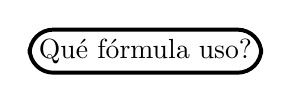
\begin{tikzpicture}
\node[draw, line width=0.5mm, rounded corners=3mm] at (8,2) {Qu\'e f\'ormula uso?};
\end{tikzpicture}
\end{frame}

\begin{frame}
\frametitle{MRU}
{\huge \xmru}

Pero.. siempre debemos trabajar en el mismo sistema de unidades.
Es decir, si hay un metros/segundos,
debemos transformar los 
minutos a segundos :)

\begin{center}
\fcolorbox{red}{white}{
\parbox[c]{6cm}{
1 minuto = 60 segundos \\
Entonces 30 minutos son \\
30 $\times$ 60 segundos \\
30 minutos =
1800 segundos.
}}
\end{center}

Finalmente..
\end{frame}

\begin{frame}
\frametitle{MRU}
{\large
\begin{equation}
x=
(5\frac{m}{\cancel{s}})
(1800~\cancel{s})=
9000~m
\end{equation}}

La distancia que recorre el ferrocarril es
\fbox{9000 m}
\end{frame}

\end{document}
%%
%% End of Beamer-ported file ==
